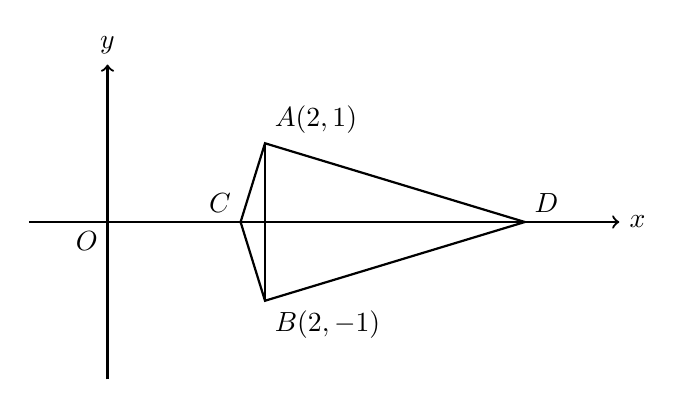
\begin{tikzpicture}[scale=1.0]
    % 绘制坐标轴
    \draw[->, thick] (-1, 0) -- (6.5, 0) node[right] {$x$};
    \draw[->, thick] (0, -2) -- (0, 2) node[above] {$y$};
    \node[below left] at (0,0) {$O$};

    % 定义点 A, B, C, D 的坐标
    % A(2,1), B(2,-1) 为 z^2-4z+5=0 的两根
    \coordinate (A) at (2, 1);
    \coordinate (B) at (2, -1);
    
    % 当 a = -7 时，z^2 - 7z + 9 = 0
    % 两个实根约为 C(1.69, 0) 和 D(5.30, 0)
    \coordinate (C) at (1.69, 0);
    \coordinate (D) at (5.30, 0);

    % 绘制四边形 ABCD
    \draw[thick] (A) -- (C) -- (B) -- (D) -- cycle;
    
    % 绘制垂直连线 AB
    \draw[thick] (A) -- (B);

    % 标注点
    \node[above right] at (A) {$A(2,1)$};
    \node[below right] at (B) {$B(2,-1)$};
    \node[above left] at (C) {$C$};
    \node[above right] at (D) {$D$};
\end{tikzpicture}